%%%%%%%%%%%%%%%%%%%%%%%%%%%%%%%%%%%%%%%%%%%%%%%%%%%%%%%%%%%%%%%%%%%%%%%%%%%%%
\section{Introduction}
\label{sec:intro}
Provided is a documentation of a recently developed Oslofjord model called FjordOs CL. It is developed as part of the project FjordOs\footnote{\texttt{http://www.fjordos.no}}. FjordOs CL is based on version 3.6 of the Regional Ocean Modeling System - ROMS \citep{haidv:etal:2008, shche:mcwil:2005, shche:mcwil:2009} utilizing its curvilinear option.

\subsection{The Oslofjord}
The Oslofjord is located in Southern Norway and is about 100 km long (Figure \ref{fig:map_oslofj}). Its width varies from about 25 km at the entrance ($\sim$ 59$^\text{o}$N) to about 1-2 km in the {\DR} Sound and {\DR} area. The fjord's main sill, which is marked by the horizontal bar in Figure \ref{fig:map_oslofj} (hereafter the {\DR} Sill), is located two thirds inside of the entrance to the fjord. This makes the Oslofjord peculiar among Norwegian fjords in that most of them have the sill at the entrance to the fjord. 
% %%%%%%%%%%%%%%%%%%%%%%%%%% Figure Map_location_Oslofjord %%%%%%%%%%%%%%%%%%%%%%%%%%%%
\begin{figure}[h]
 \setlength{\unitlength}{1.0cm}
 \begin{center}
  \begin{pspicture}(0,0)(15,9)
% Include graphs
   \rput[bl](-0.1,1.0){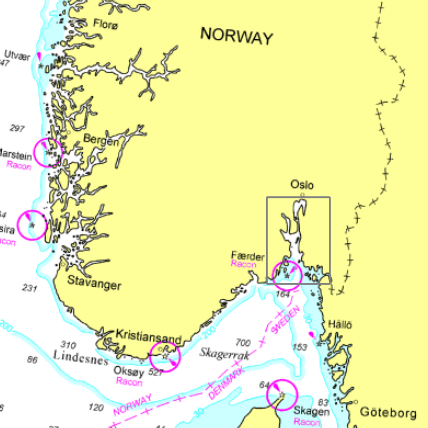
\includegraphics[height=7.3cm]{Map_location_Oslofjord_2}}
   \rput[br](15.0,0.0){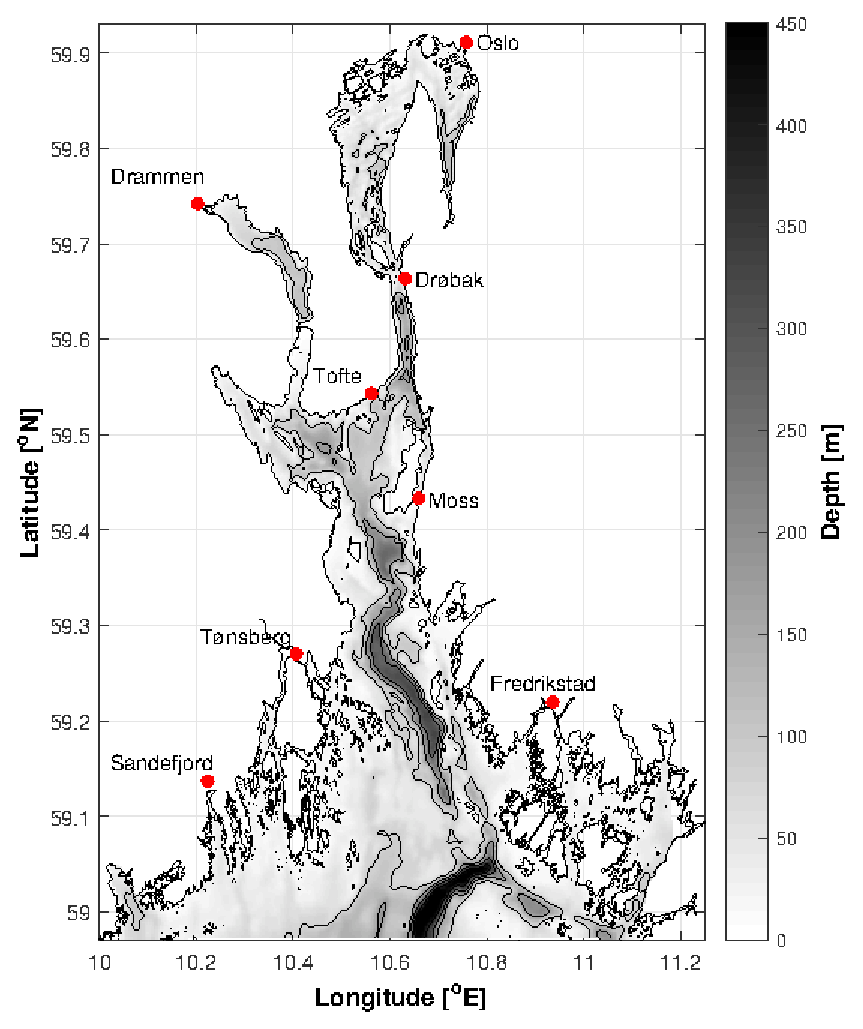
\includegraphics[height=9cm]{dyp_old}}
   \psline[linewidth=0.5mm,linecolor=blue]{->}(13.4,5.3)(11.3,6.3)
   \psline[linewidth=0.2mm](4.45,4.95)(7.5,8.5)
   \psline[linewidth=0.2mm](4.45,3.5)(7.5,1)
  \end{pspicture}
% Figure caption is below the figure
  \caption{\small The topography and irregular coastline of the Oslofjord and its location in Southern Norway. The right-hand gray scale bar indicates depth in meters. The blue arrow points to the location of the fjord's main sill (the {\DR} sill as enlarged in Figure \ref{fig:droebak_sill}) which is only $\sim$ 20 m deep. Note also the $\sim$ 400 m deep basin extending from the Skagerrak towards the Hvaler Archipelago in the southeast, the so called Hvalerdjupet. }
  \label{fig:map_oslofj}       % Give a unique label
 \end{center}
\end{figure}
%


The {\DR} Sill is partly man made\footnote{The jetty was built in the years 1874 - 1879 as a naval defense of Oslo, the capital of Norway. It forces large vessels to sail east of the fortress Oscarsborg built at Kaholmen.} and partly natural. The natural sill is about 20 m deep, while the man made part is only 1-2 m deep. The latter consists of an underwater barrier, the {\DR} Jetty, extending halfway across the {\DR} Sound from the western mainland south of {\DR} to south of the small island Kaholmen located slightly to the east of the southern tip of the {\HAA} (Figure \ref{fig:droebak_sill}). There are two narrow openings in the Jetty with a maximum depth of about 6 m. One is located close to the mainland on the western side, while the second runs east-west and is located just south of Kaholmen.   
%%%%%%%%%%%%%%%%%%% Figure 2 Bathymetry and currents in the Drøbak area %%%%%%%%%%%%%%%
\begin{figure}[t]
 \begin{center}
  \begin{pspicture}(0,0)(15,9)
% Include graphs
   \rput[b](7.5,0){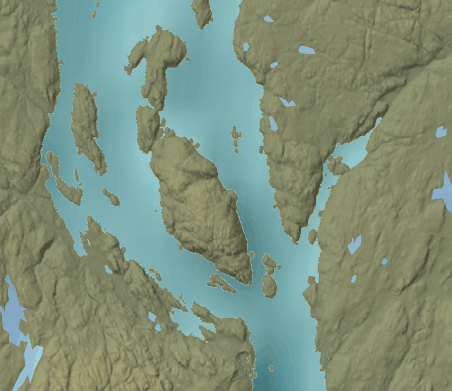
\includegraphics[height=9cm]{dyp_Drobak}}
   \rput[b](11,0){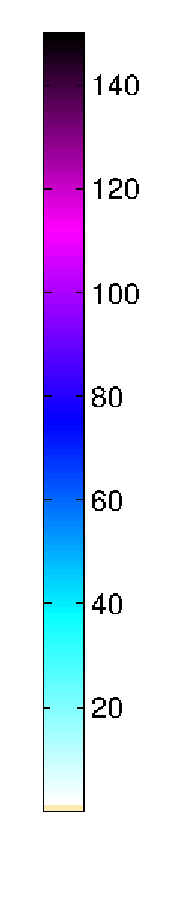
\includegraphics[height=9cm]{Fig02_color_bar}}
  \end{pspicture}
  \caption{\small The irregular coastline and topography in the {\DR} Sill area. The color bar indicates depth in meters.}
  \label{fig:droebak_sill}
 \end{center}
\end{figure}

 

The sill area represent a major obstruction for the water exchange between the inner and the outer part of the fjord. Due its narrowness and shallowness the {\DR} Sill area is famous for its strong tidal currents that can be as swift as 1 m/s. We also note that north of the sill the fjord is separated by {\HAA} into an eastern and a western channel each about 1 km wide. These channels and the openings in the Jetty are important to include in any model of the Oslofjord to obtain realistic circulation patterns and strengths in the area. Another noteworthy topographic feature is the Hvalerdjup located at the entrance to the fjord (Figures \ref{fig:map_oslofj} and \ref{fig:ferder_hvaler}). It is a 400 m deep basin extending northeastward from the Skagerrak towards the Hvaler Archipelago. As revealed by Figure \ref{fig:map_oslofj} there are also several other somewhat shallower basins $\sim$ 150 - 200 m deep as we proceed into the fjord. 
%%%%%%%%%%%%%%%%%%% Figure 2 Bathymetry and currents in the Drøbak area %%%%%%%%%%%%%%%
\begin{figure}[t]
 \begin{center}
  \begin{pspicture}(0,0)(15,8.5)
% Include graphs
   \rput[bl](-0.1,0){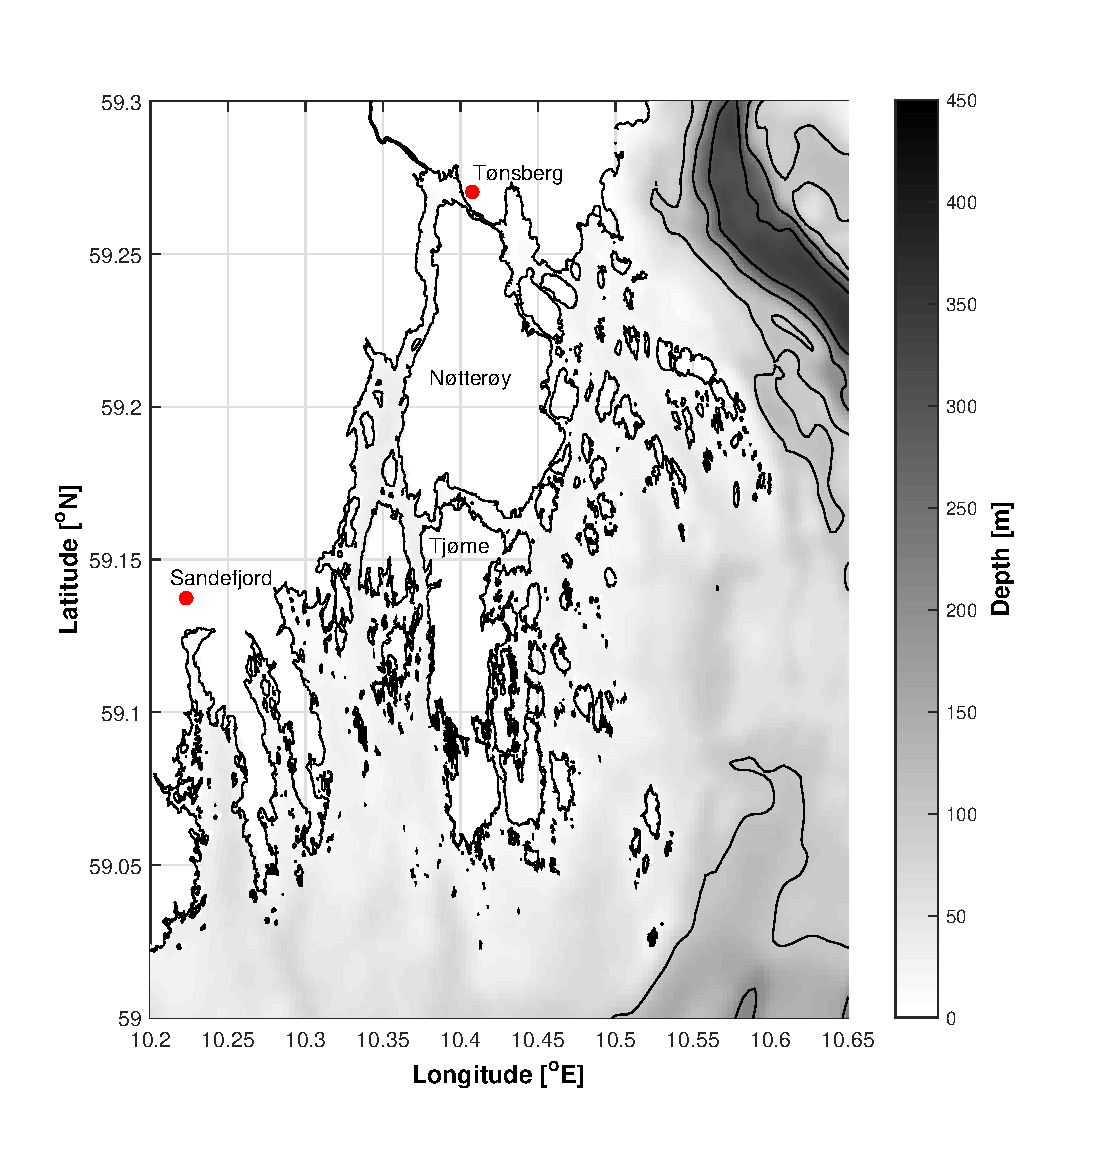
\includegraphics[height=8.5cm]{dyp_Tonsberg}}
   \rput[bl](7.5,0){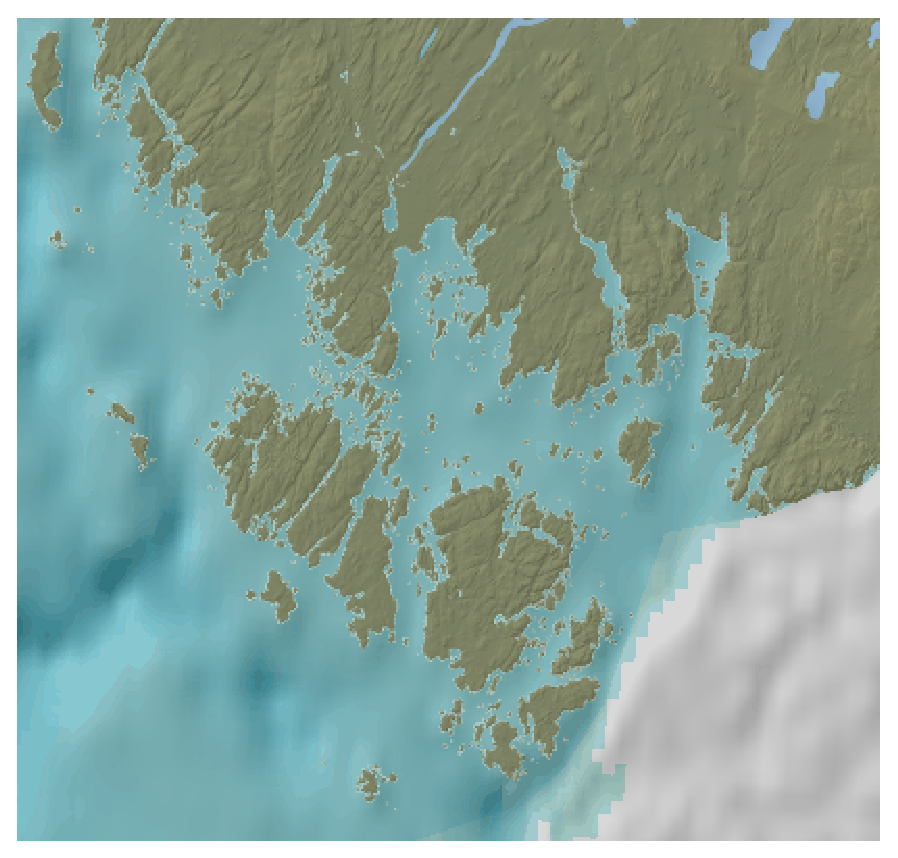
\includegraphics[height=8.5cm]{dyp_Hvaler}}
   \rput[bl](0,7){\large \textbf{a)}}
   \rput[bl](7.5,7){\large \textbf{b)}}
  \end{pspicture}
  \caption{\small a) The irregular coastline geometry and topography in the a) F{\ae}rder National Park and b) the Hvaler National Park. The grayscale in color bars indicates depth in meters. Note the many islands, narrow straits and channels present in these areas of the Oslofjord.}
  \label{fig:ferder_hvaler}
 \end{center}
\end{figure}

 

In addition to the {\DR} Sill area there are other areas in the fjord that features many smaller and larger islands. For instance to the west we find the T{\o}nsberg Archipelago including Bol{\ae}rne, Store and Lille F{\ae}rder (F{\ae}rder Lighthouse), and to the east we find Rau{\o}y and Hank{\o} including the smaller Island S{\o}strene and Misingene and the Hvaler Archipelago (Figure \ref{fig:ferder_hvaler}). Further north on the west side of the fjord we find Bast{\o} south of Horten, and to the east Jel{\o}ya just west of Moss. Jel{\o}ya is separated from the mainland by a narrow channel about 50 m wide within which water sloshes back and forth with the tides \citep{hjelm:etal:2014}. The presence of these archipelagos with its small islands give rise to many narrow sounds, straits and channels impeding the water exchange. If the goal is to compute realistic pathways of any unwanted substances discharged to the fjord or trajectories of floating structures including man overboard (Search and Rescue Services), we need to resolve, to the best of our ability, these features. 

Finally it is worth mentioning the many rivers discharge freshwater to the fjord. For instance two of Norway's largest rivers, namely Glomma and Drammenselva\footnote{Here it is chosen to use Norwegian river names in which ``elv'' or ``vassdrag'', means ``river'' or ``water course''.}, are emptying their freshwater into the Oslofjord with a mean discharge of 729 and 317 m$^3$/s, respectively \citep{milli:etal:2011}. This freshwater has a decisive impact on the salinity and hence on the circulation in the fjord. Furthermore, in most fjords the river outlet is located at the fjord head leading to an estuarine circulation. In contrast the Glomma outlet is located in the outer part of the Oslofjord within the Hvaler Archipelago, while the Drammenselva outlet is located in the middle part of the fjord. As a result the estuarine circulation in the Oslofjord deviates considerably from a classical textbook example.        
%%%%%%%%%%%%%%%%%%%%%%%%%%% Figure 3 Godafoss %%%%%%%%%%%%%%%%%%%%%%%%%%%%%%%
\begin{figure}[t]
 \begin{center}
  \begin{pspicture}(0,0)(15,5.5)
% Include graphs
   \rput[bl](0.0, 0.0){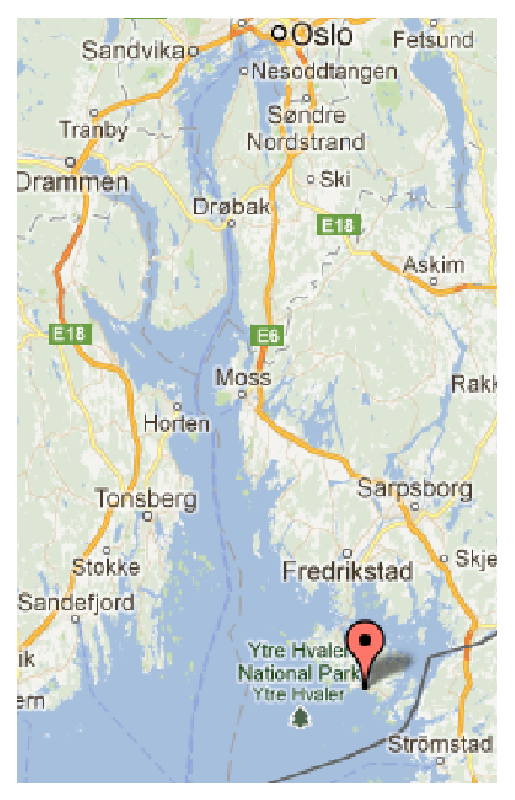
\includegraphics[height=5.5cm]{Fig03}}
   \rput[br](15.0,0.0){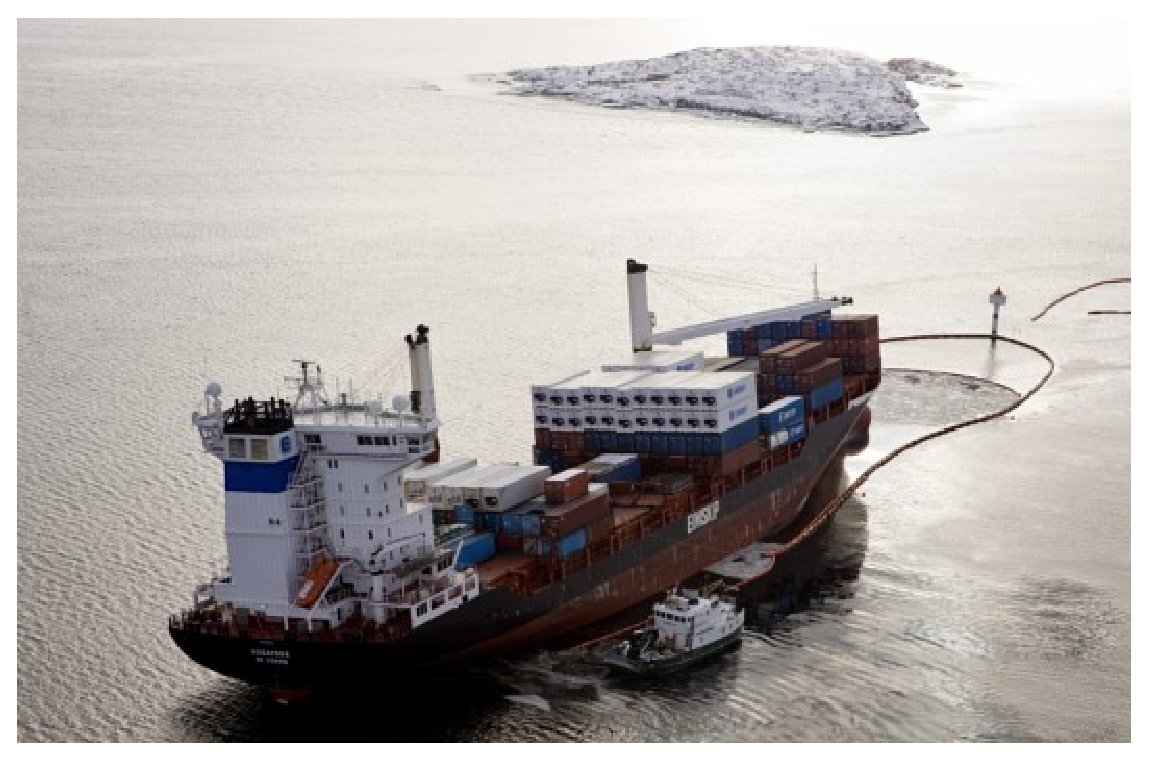
\includegraphics[height=5.5cm]{Fig03_2}}
  \end{pspicture}
  \caption{\small Map (left) showing the location where the ship ``Godafoss'' (right) grounded February 17, 2011. The location is in the sound L{\o}peren between two of the major islands in the Hvaler Archipelago where Norway's largest river flows through on its way to the Oslofjord.} 
  \label{fig:godafoss}
 \end{center}
\end{figure}



% % % % % % % % % % % % % % % % % % % % % % % % % % % % % % % % 
\subsection{Why a new model?}
The Oslofjord is somewhat special among the Norwegian fjords from a physical as well as a societal perspective. The population surrounding it, or more precisely people living less than one hours drive from the Oslofjord, comprises 40\% of the Norwegian population according to the official statistics\footnote{\texttt{http://www.ssb.no} as of July 1, 2012}. This is by far the most populated area in Norway, a population that is steadily growing. Moreover, no other fjord has anything close to as high density of leisure boats. In addition the Oslofjord features two of Norway's national underwater parks, the Hvaler National Park\footnote{\texttt{http://www.ytrehvaler.no/}} and the F{\ae}rder National Park\footnote{\texttt{http://prosjekt.fylkesmannen.no/faerdernasjonalpark/Om-Farder-nasjonalpark/}}. Thus, taking into account that the Oslofjord has the largest traffic density of commercial vessels of all the Norwegian fjords the risk of an accident resulting in a possible, unwanted contaminated effluent to the fjord is uncomfortably high. 
%%%%%%%%%%%%%%%%%%%%%%%%%%% Figure 3 Godafoss %%%%%%%%%%%%%%%%%%%%%%%%%%%%%%%
\begin{figure}[t]
 \begin{center}
  \begin{pspicture}(0,0)(15,10)
% Include graphs
   \rput[b](7.7, 0.0){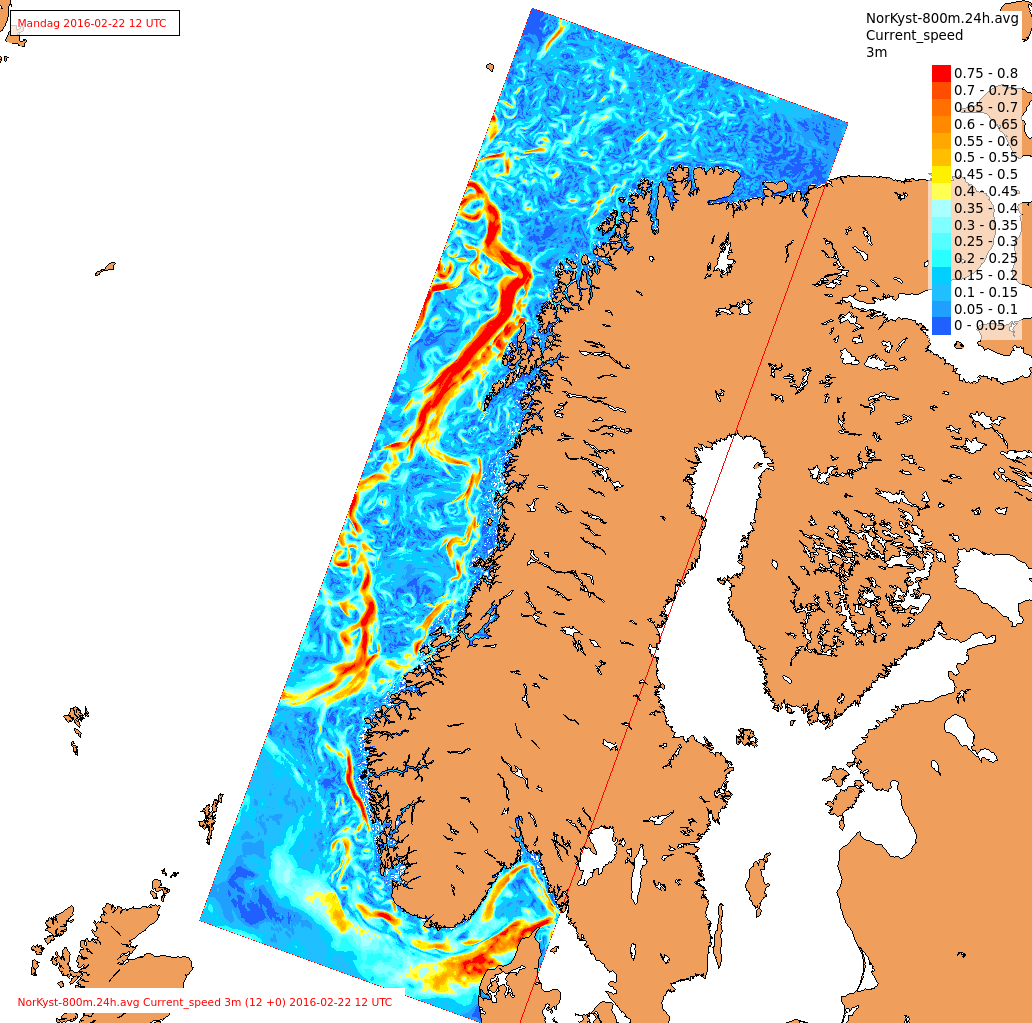
\includegraphics[height=10cm]{N800_2016-02-22_SPEED_3m_24h_avg}}
  \end{pspicture}
  \caption{\small The area covered by the NorKyst800 model. Shown is forecasted, 24 hour average speed at 3 m depth valid for February 22, 2016. Color bar gives speed in m/s with a a contour interval of 0.05 m/s.} 
  \label{fig:n800}
 \end{center}
\end{figure}

 

An example of such an unwanted event is the Godafoss accident. On February 17, 2011 the ship ``Godafoss'' grounded in a narrow sound in the Hvaler Archipelago (Figure \ref{fig:godafoss}). As a result a lot of its fuel oil was discharged into the fjord. When an event like this happens MET Norway has to, within half an hour, forecast the dispersion, drift and spreading of the oil as part of its emergency preparedness\footnote{On behalf of the Norwegian Coastal Administration (Kystverket)}. Recall that most of the accidents like Godafoss tend to happen within archipelagos\footnote{\texttt{https://en.wikipedia.org/wiki/List\_of\_oil\_spills}}. The safety of the people that utilize the fjord, and the protection of its environment, is therefore a challenge to governmental agencies, regional administrations and local management alike. 

One of the key inputs to the emergency preparedness models for oil drift is ocean currents and temperature together with wave and atmospheric input. The present model providing forecasts of ocean currents and temperature for the Oslofjord, and which is run operationally by MET Norway on a 24/7 basis, is the NorKyst800 model \citep{albre:etal:2011}. As depicted by Figure \ref{fig:n800} it covers not only the Oslofjord, but actually the entire Norwegian coast. It was developed to capture mesoscale phenomena such as jet currents, eddies and meanders in Norway's near coastal areas, and to provide forecasts of some reliability in the fjords. It was set-up with a regular grid of 800x800 m, a grid of high enough resolution to resolve the Rossby radius of deformation required to capture the mesoscale phenomena in Norway's near coastal waters. 
%%%%%%%%%%%%%%%%%%%%%%%%%%% Figure 3 Godafoss %%%%%%%%%%%%%%%%%%%%%%%%%%%%%%%
\begin{figure}[t]
 \begin{center}
  \begin{pspicture}(0,0)(15,5.2)
% Include graphs
   \rput[bl]( 0.0,0.0){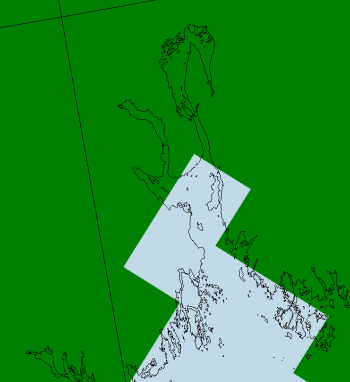
\includegraphics[height=5.2cm]{Oslofjord_A20_grid}}
   \rput[b ]( 7.5,0.0){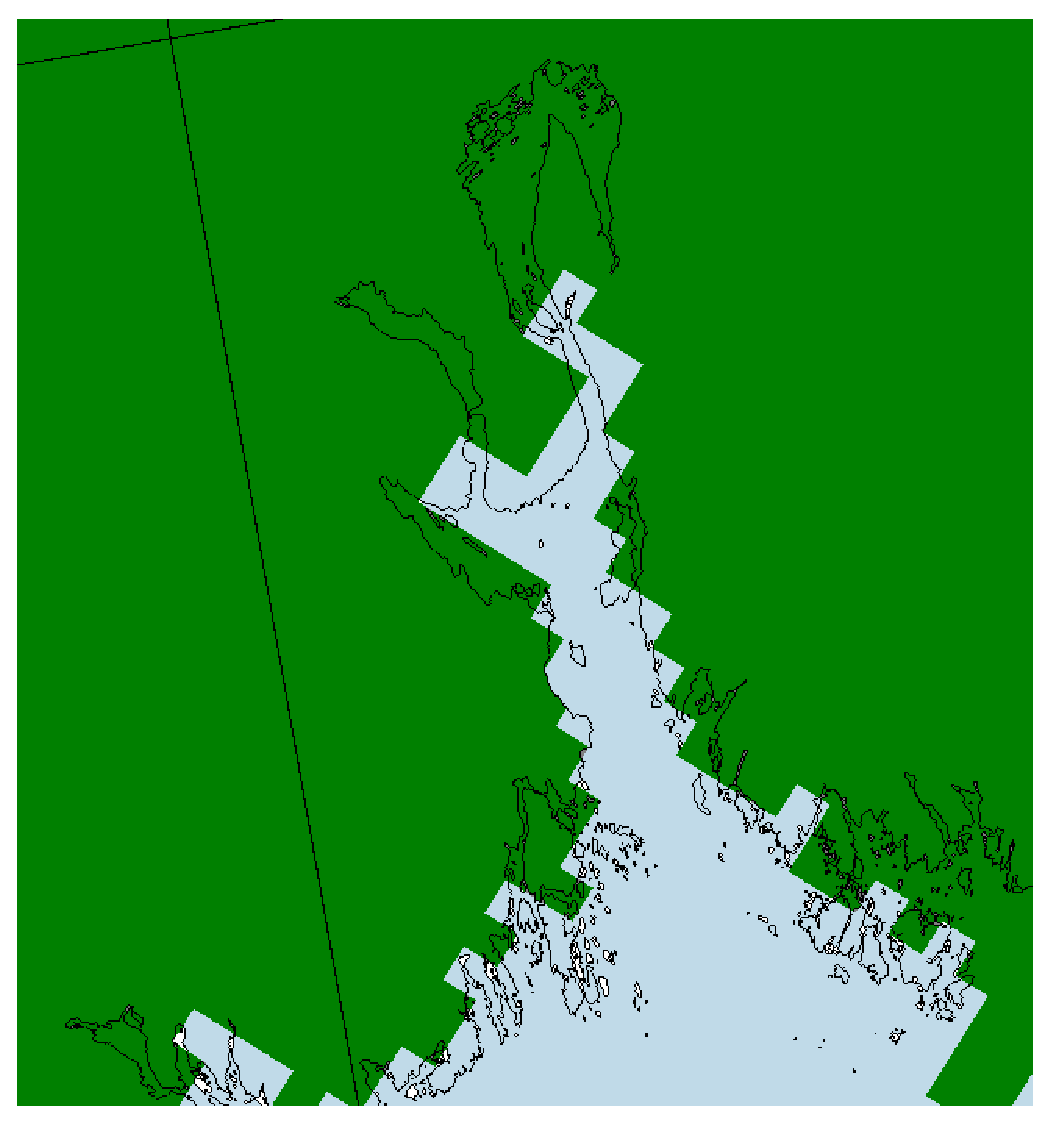
\includegraphics[height=5.2cm]{Oslofjord_N4_grid}}
   \rput[br](15.0,0.0){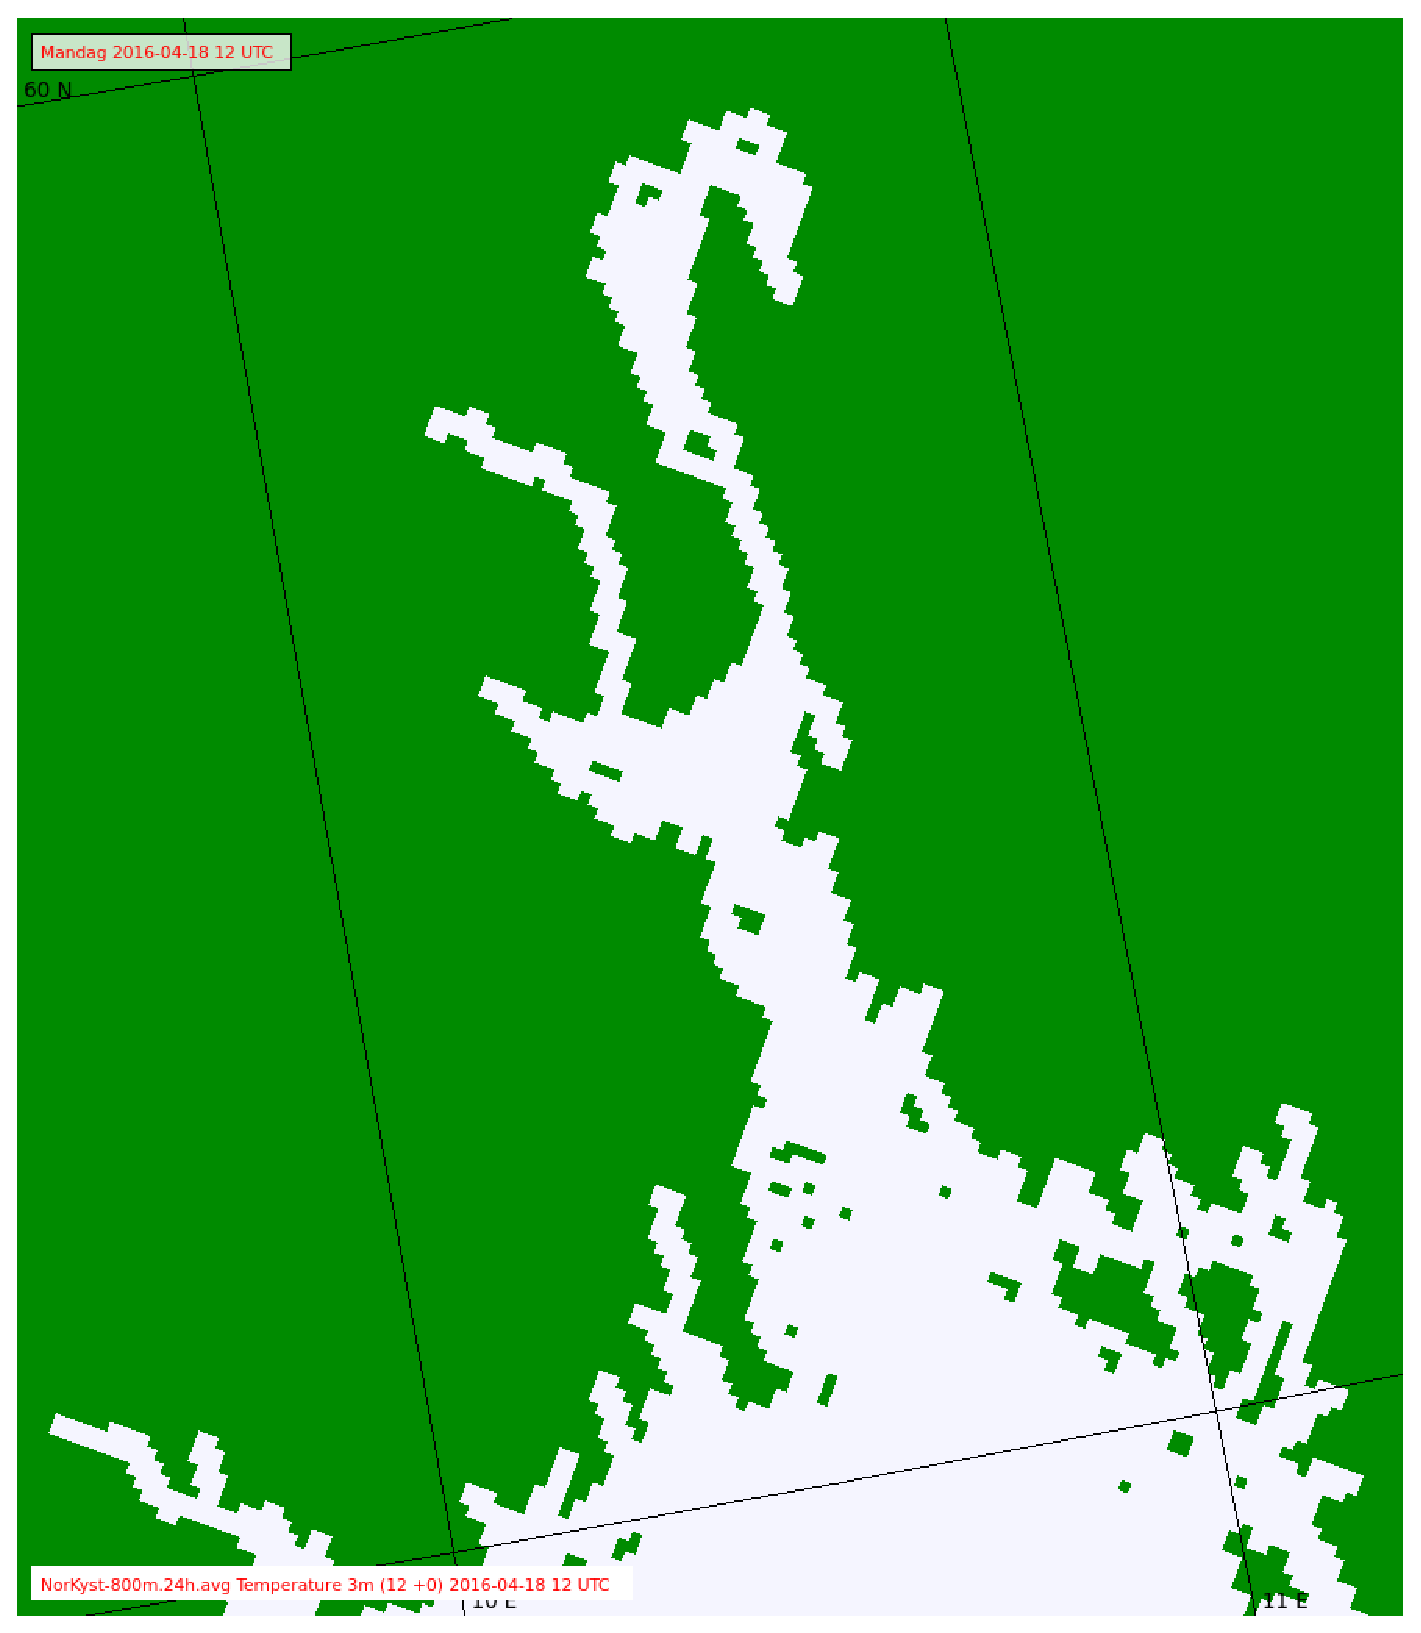
\includegraphics[height=5.2cm]{Oslofjord_N800_grid}}
   \rput[bl]( 0.3,4.7){\large \textbf{a)}}
   \rput[b ]( 5.6,4.7){\large \textbf{b)}}
   \rput[br](10.9,4.7){\large \textbf{c)}}
  \end{pspicture}
  \caption{\small Map of the Oslofjord overlayed by a 20 km grid size (a), 4 km grid size (b) and 800 m grid size (c) model.} 
  \label{fig:resolution}
 \end{center}
\end{figure}



Nevertheless the resolution offered by NorKyst800 is not fine enough to resolve the highly irregular geometry and topography of most Norwegian fjords, and the Oslofjord is no exception. These irregularities consist of small islands, narrow sounds, straits and channels and many smaller scale deep basins and shallow sills (Figure \ref{fig:map_oslofj}). To properly be prepared to forecast the transport and spreading of any unwanted substances or contaminants accidentally discharged to the fjord it is of importance that the underlying fjord model resolves the \emph{sub}mesocale phenomena generated by the presence of these irregularities, in addition to resolve the mesoscale phenomena. We emphasize that such a model, when operational, will benefit all emergency preparedness models that is operated by MET Norway. Examples of such models are, in addition to oil drift, (i) Search And Rescue (SAR) which involves forecasting of pathways of floating objects such as man overboard, rafts, small crafts and ships, (ii) transport and spreading of dissolved substances such as nutrients, nuclear waste and other dissolved toxic substances, and (iii) growth and drift of toxic algae. Finally we emphasize that resolving the submesoscale motion due to the fjord's irregular geometry and topography is required to avoid floating objects, dissolved substances and oil from stranding artificially.  

How the resolution impacts on how well the model portrays these irregularities is perhaps best illustrates by Figures \ref{fig:resolution} and \ref{fig:resolution_2}. The former shows how the Oslofjord is depicted in, respectively, a 20 km, 4 km and 800 m grid, while the latter, focusing on an enlargement of the area between {\DR} and T{\o}nsberg, depicts how the fjord is portrayed in, respectively, a 4 km, 800 m and 100 m grid. As is evident from Figure \ref{fig:resolution} it is only the 100 m grid that represents the fjord as something that looks like the Oslofjord geometry as we know it from geographical charts and maps. Zooming in on Breidangen (Figure \ref{fig:resolution_2}) we observe that it takes at least a 100 m grid to properly represent the many narrow straits, channels and islands present in the fjord. For instance we note the presence of small islands in Breidangen present in the 100 m grid which is simply not there in the 800 m grid. Likewise the shape and area covered by Bast{\o}y is improved in the 100 m grid, and so is the ridge that cuts into the the Drammensfjord at Svelvik. The same is true regarding topography as displayed in Figure \ref{fig:hvaler2} comparing the Hvalerdjupet in the NorKyst800 model with the 100 m resolution topography. 
%%%%%%%%%%%%%%%%%%%%%%%%%%% Figure 3 Godafoss %%%%%%%%%%%%%%%%%%%%%%%%%%%%%%%
\begin{figure}[t]
 \begin{center}
  \begin{pspicture}(0,0)(15,6.5)
% Include graphs
   \rput[bl]( 0.0,0.0){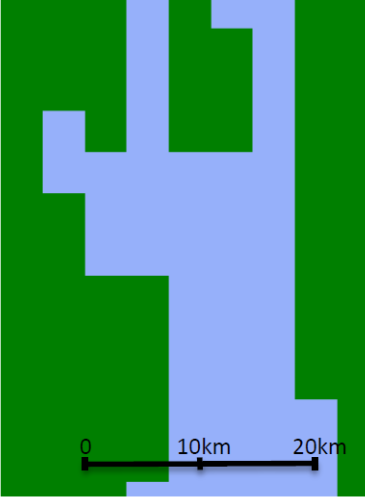
\includegraphics[height=6.5cm]{Midfjord_N4_grid}}
   \rput[b ]( 7.5,0.0){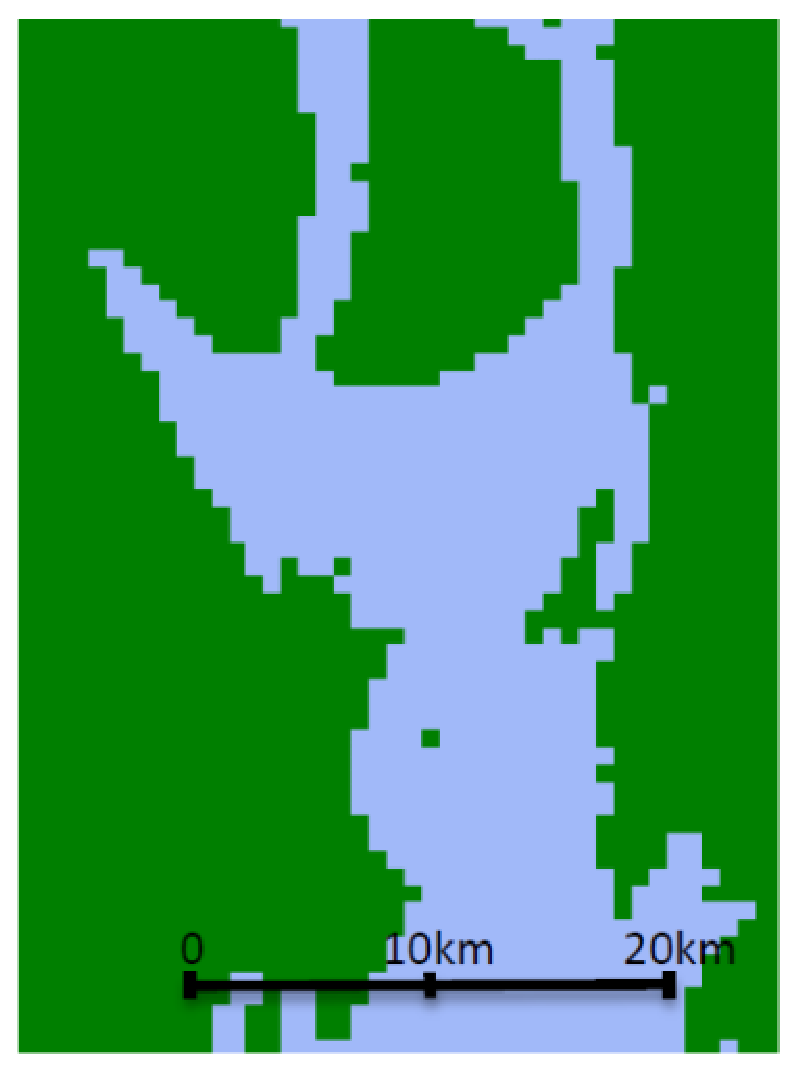
\includegraphics[height=6.5cm]{Midfjord_N800_grid}}
   \rput[br](15.0,0.0){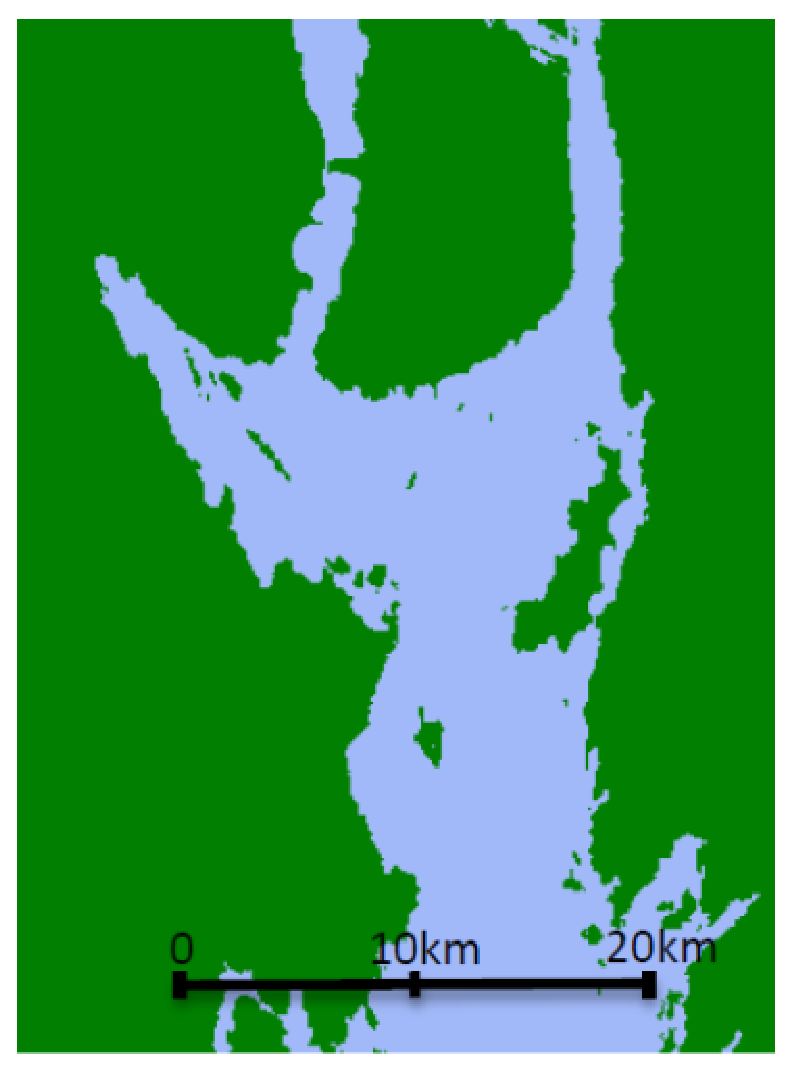
\includegraphics[height=6.5cm]{Midfjord_100m_grid}}
   \rput[bl]( 0.3,6.0){\large \textbf{a)}}
   \rput[b ]( 5.6,6.0){\large \textbf{b)}}
   \rput[br](10.9,6.0){\large \textbf{c)}}
  \end{pspicture}
  \caption{\small As Figure \ref{fig:resolution}, but zoomed in on Breidangen. To better reveal the grid the underlying map is not shown. (a) 4 km grid, (b) 800 m grid and (c) 100 m grid. Note that it takes a 100 m grid to properly resolve the many islands, narrow straits and channels present in the fjord. } 
  \label{fig:resolution_2}
 \end{center}
\end{figure}



To conclude the present forecasting models for the Oslofjord (NorKyst800) has an insufficient resolution, and a new model of the Oslofjord with a resolution of 100 m or less, at least in parts of the fjord, is in need. The development of a such a model would also greatly benefit the other emergency preparedness products delivered by MET Norway on behalf of other governmental institutions and agencies, e.g., the Norwegian Coastal Administration (Kystverket) and the Norwegian Radiation Protection Authorities (NRPA).   
%%%%%%%%%%%%%%%%%%% Figure 2 Bathymetry and currents in the Drøbak area %%%%%%%%%%%%%%%
\begin{figure}[t]
 \begin{center}
  \begin{pspicture}(0,0)(15,8.5)
% Include graphs
   \rput[tl](-0.1,9.5){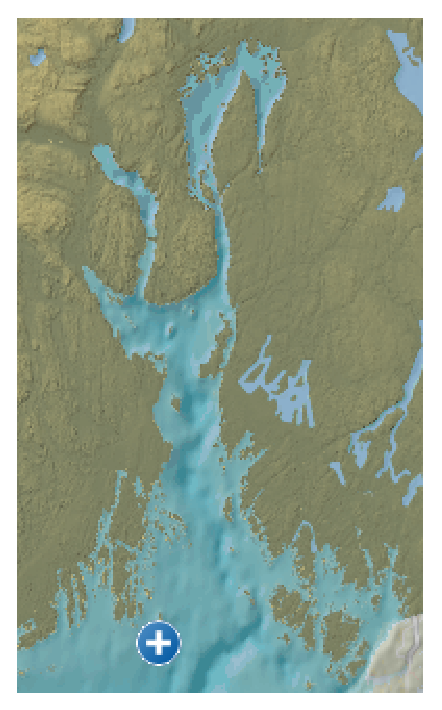
\includegraphics[height=8.5cm]{dyp}}
   \rput[tr](  15,9.5){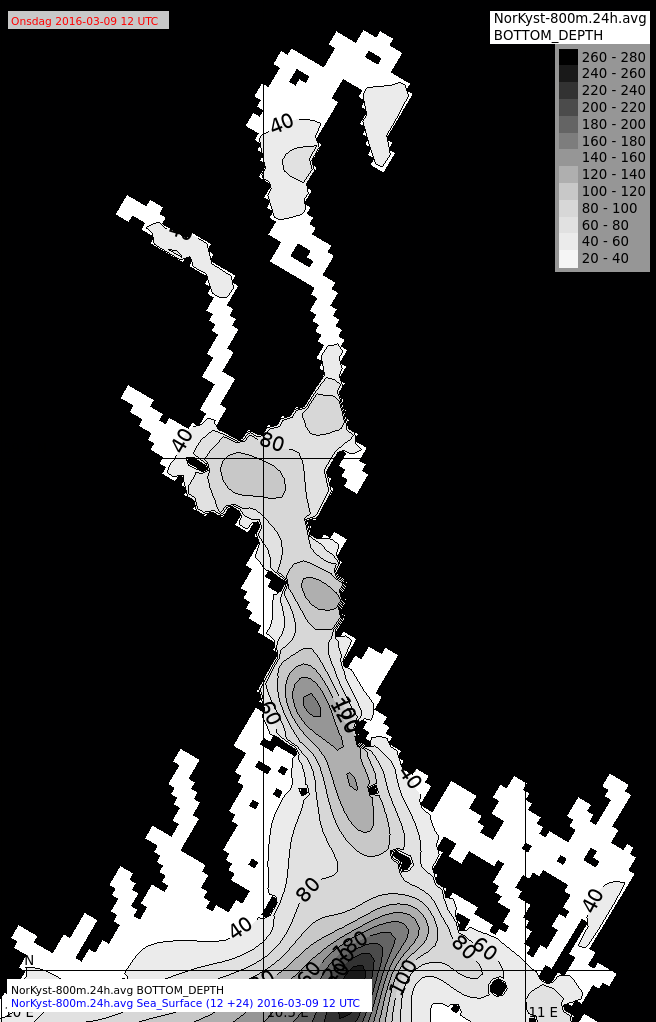
\includegraphics[height=8.0cm]{NorKyst800_topo_oslofjord}}
  \end{pspicture}
  \caption{\small The irregular coastline geometry and topography in the Oslofjord as portrayed in the FjordOs CL model (left) and the NorKyst800 model (right). The color bar (grayscale) indicate depth in meters.}
  \label{fig:hvaler2}
 \end{center}
\end{figure}



% % % % % % % % % % % % % % % % % % % % % % % % % % % % % % % % 
\subsection{Organization of the report}
The report is organized as follows. Section \ref{sec:model} provides some details on how the curvilinear grid of the FjordOs CL model is constructed. Section \ref{sec:setup} provides some model specifics while Section \ref{sec:forcing} gives details on the model's bathymetry and external forcing such as tides, ocean input through open lateral boundaries, river input as well as atmospheric input. Section \ref{sec:resul} provides some results from an almost two year long hindcast and some test forecasts. Finally we offer a summary and some concluding remarks in Section \ref{sec:summa}. 
